% Template for PLoS
% Version 3.6 Aug 2022
%
% % % % % % % % % % % % % % % % % % % % % %
%
% -- IMPORTANT NOTE
%
% This template contains comments intended 
% to minimize problems and delays during our production 
% process. Please follow the template instructions
% whenever possible.
%
% % % % % % % % % % % % % % % % % % % % % % % 
%
% Once your paper is accepted for publication, 
% PLEASE REMOVE ALL TRACKED CHANGES in this file 
% and leave only the final text of your manuscript. 
% PLOS recommends the use of latexdiff to track changes during review, as this will help to maintain a clean tex file.
% Visit https://www.ctan.org/pkg/latexdiff?lang=en for info or contact us at latex@plos.org.
%
%
% There are no restrictions on package use within the LaTeX files except that no packages listed in the template may be deleted.
%
% Please do not include colors or graphics in the text.
%
% The manuscript LaTeX source should be contained within a single file (do not use \input, \externaldocument, or similar commands).
%
% % % % % % % % % % % % % % % % % % % % % % %
%
% -- FIGURES AND TABLES
%
% Please include tables/figure captions directly after the paragraph where they are first cited in the text.
%
% DO NOT INCLUDE GRAPHICS IN YOUR MANUSCRIPT
% - Figures should be uploaded separately from your manuscript file. 
% - Figures generated using LaTeX should be extracted and removed from the PDF before submission. 
% - Figures containing multiple panels/subfigures must be combined into one image file before submission.
% For figure citations, please use "Fig" instead of "Figure".
% See http://journals.plos.org/plosone/s/figures for PLOS figure guidelines.
%
% Tables should be cell-based and may not contain:
% - spacing/line breaks within cells to alter layout or alignment
% - do not nest tabular environments (no tabular environments within tabular environments)
% - no graphics or colored text (cell background color/shading OK)
% See http://journals.plos.org/plosone/s/tables for table guidelines.
%
% For tables that exceed the width of the text column, use the adjustwidth environment as illustrated in the example table in text below.
%
% % % % % % % % % % % % % % % % % % % % % % % %
%
% -- EQUATIONS, MATH SYMBOLS, SUBSCRIPTS, AND SUPERSCRIPTS
%
% IMPORTANT
% Below are a few tips to help format your equations and other special characters according to our specifications. For more tips to help reduce the possibility of formatting errors during conversion, please see our LaTeX guidelines at http://journals.plos.org/plosone/s/latex
%
% For inline equations, please be sure to include all portions of an equation in the math environment.  For example, x$^2$ is incorrect; this should be formatted as $x^2$ (or $\mathrm{x}^2$ if the romanized font is desired).
%
% Do not include text that is not math in the math environment. For example, CO2 should be written as CO\textsubscript{2} instead of CO$_2$.
%
% Please add line breaks to long display equations when possible in order to fit size of the column. 
%
% For inline equations, please do not include punctuation (commas, etc) within the math environment unless this is part of the equation.
%
% When adding superscript or subscripts outside of brackets/braces, please group using {}.  For example, change "[U(D,E,\gamma)]^2" to "{[U(D,E,\gamma)]}^2". 
%
% Do not use \cal for caligraphic font.  Instead, use \mathcal{}
%
% % % % % % % % % % % % % % % % % % % % % % % % 
%
% Please contact latex@plos.org with any questions.
%
% % % % % % % % % % % % % % % % % % % % % % % %

\documentclass[10pt,letterpaper]{article}
\usepackage[top=0.85in,left=2.75in,footskip=0.75in]{geometry}

% amsmath and amssymb packages, useful for mathematical formulas and symbols
\usepackage{amsmath,amssymb}

% Use adjustwidth environment to exceed column width (see example table in text)
\usepackage{changepage}

% textcomp package and marvosym package for additional characters
\usepackage{textcomp,marvosym}

% cite package, to clean up citations in the main text. Do not remove.
\usepackage{cite}

% Use nameref to cite supporting information files (see Supporting Information section for more info)
\usepackage{nameref,hyperref}
\usepackage[normalem]{ulem}
% line numbers
\usepackage[right]{lineno}

% ligatures disabled
\usepackage[nopatch=eqnum]{microtype}
\DisableLigatures[f]{encoding = *, family = * }

% color can be used to apply background shading to table cells only
\usepackage[table]{xcolor}

% array package and thick rules for tables
\usepackage{array}

% create "+" rule type for thick vertical lines
\newcolumntype{+}{!{\vrule width 2pt}}

% create \thickcline for thick horizontal lines of variable length
\newlength\savedwidth
\newcommand\thickcline[1]{%
  \noalign{\global\savedwidth\arrayrulewidth\global\arrayrulewidth 2pt}%
  \cline{#1}%
  \noalign{\vskip\arrayrulewidth}%
  \noalign{\global\arrayrulewidth\savedwidth}%
}

% \thickhline command for thick horizontal lines that span the table
\newcommand\thickhline{\noalign{\global\savedwidth\arrayrulewidth\global\arrayrulewidth 2pt}%
\hline
\noalign{\global\arrayrulewidth\savedwidth}}


% Remove comment for double spacing
%\usepackage{setspace} 
%\doublespacing

% Text layout
\raggedright
\setlength{\parindent}{0.5cm}
\textwidth 5.25in 
\textheight 8.75in

% Bold the 'Figure #' in the caption and separate it from the title/caption with a period
% Captions will be left justified
\usepackage[aboveskip=1pt,labelfont=bf,labelsep=period,justification=raggedright,singlelinecheck=off]{caption}

\renewcommand{\figurename}{Fig}

% Use the PLoS provided BiBTeX style
\bibliographystyle{plos2015}

% Remove brackets from numbering in List of References
\makeatletter
\renewcommand{\@biblabel}[1]{\quad#1.}
\makeatother



% Header and Footer with logo
\usepackage{lastpage,fancyhdr,graphicx}
\usepackage{epstopdf}
%\pagestyle{myheadings}
\pagestyle{fancy}
\fancyhf{}
%\setlength{\headheight}{27.023pt}
%\lhead{\includegraphics[width=2.0in]{PLOS-submission.eps}}
\rfoot{\thepage/\pageref{LastPage}}
\renewcommand{\headrulewidth}{0pt}
\renewcommand{\footrule}{\hrule height 2pt \vspace{2mm}}
\fancyheadoffset[L]{2.25in}
\fancyfootoffset[L]{2.25in}
\lfoot{\today}

%% Include all macros below

\newcommand{\lorem}{{\bf LOREM}}
\newcommand{\ipsum}{{\bf IPSUM}}

%% END MACROS SECTION


\begin{document}
\vspace*{0.2in}

% Title must be 250 characters or less.
\begin{flushleft}
{\Large
\textbf\newline{Untangling temporal signal for calibrating the molecular clock of microbes} % Please use "sentence case" for title and headings (capitalize only the first word in a title (or heading), the first word in a subtitle (or subheading), and any proper nouns).
}
\newline
% Insert author names, affiliations and corresponding author email (do not include titles, positions, or degrees).
\\
John H Tay\textsuperscript{1},
Arthur Kocher\textsuperscript{2,3},
Sebastian Duchene\textsuperscript{1,4,*},
\\
\bigskip
\textbf{1} Peter Doherty Institute for Infection and Immunity, Department of Microbiology and Immunology, University of Melbourne, Melbourne, Australia
\\
\textbf{2} Transmission, Infection, Diversification and Evolution Group, Max Planck Institute of Geoanthropology, Jena, Germany.
\\
\textbf{3} Department of Archaeogenetics, Max Planck Institute for Evolutionary Anthropology, Leipzig, Germany.
\\
\textbf{4} Department of Computational Biology, Institut Pasteur, Paris, France
\\
\bigskip

% Insert additional author notes using the symbols described below. Insert symbol callouts after author names as necessary.
% 

% \textcurrency b Insert second current address 
% \textcurrency c Insert third current address

% Use the asterisk to denote corresponding authorship and provide email address in note below.
* sduchene@pasteur.fr

\end{flushleft}
% Please keep the abstract below 300 words
\section*{Abstract}
Our understanding of the evolution of many microbes has been revolutionised by the molecular clock, a statistical procedure used to infer evolutionary rates and timescales from the comparative analysis of biomolecular sequences. The fundamental assumption of molecular clock models is that the rate at which substitutions accumulate can be described by a statistical process. In all molecular clock models, evolutionary rates and times are jointly unidentifiable and 'calibration' information is therefore required.

For many microbes, the sequence sampling times themselves can be often used for calibration. Phylogenetic tests of temporal signal are used to decide whether such calibrations are reliable. Critically, in addition to the calibration information, the full Bayesian phylogenetic model also includes the molecular clock model and a branching process (tree prior). As a result, there are multiple sources of information that are difficult to untangle.

We assessed temporal signal in three microbial pathogen data sets with a range of evolutionary characteristics and with ancient DNA sequences; \textit{Powassan virus} (POWV), the cholera bacetrium (\textit{Vibrio cholerae}), and the syphilis bacterium (\textit{Treponema palladium.}). We found that the tree prior can have a substantial impact on whether temporal signal is detected. To investigate this problem simulated data under several conditions and calculated the sensitivity and specificity of these tests of temporal signal under several tree priors. Highly informative sequence data sets with clear temporal signal are generally robust to the tree prior. However, in data sets with low information content of where there is no temporal signal, choosing a prior that is highly informative and inconsistent with the data can result in the false rejection of temporal signal. 

We demonstrate that prior sensitivity analyses and prior predictive simulations are an effective means to determine whether the prior is reasonable and to improve the detection of temporal signal and leverage the information that can be drawn from molecular sequence data sets.


% Please keep the Author Summary between 150 and 200 words
% Use first person. PLOS ONE authors please skip this step. 
% Author Summary not valid for PLOS ONE submissions.   
\section*{Author summary}
Molecular sequence data have become essential to infer organisms' evolutionary relationships and timescales via molecular clock models. In particular, our knowledge of when historical and modern pathogens emerged and spread is largely grounded on molecular clock models. These inferences, however, assume that sequence sampling times must have captured a sufficient amount of evolutionary change, which is typically determined using tests of temporal signal, such as the Bayesian Evaluation of Temporal Signal, BETS. Although BETS is generally effective, here we show that it can incorrectly detect temporal signal if the chosen/specified evolutionary model makes implausible statements about the evolutionary time-scale, a situation that is difficult to diagnose, particularly with complex Bayesian models. We demonstrate that this problem is due to a statistical artefact, that we refer to as tree extension and that it can be minimised by conducting careful prior predictive simulations, and by eliciting biologically plausible priors in the model. Overall, our study provides guidelines for improving our statistical confidence in estimates of evolutionary time-scales, with key applications for recently emerging pathogens and data sets involving ancient molecular data.

\linenumbers

% Use "Eq" instead of "Equation" for equation citations.
\section*{Introduction}
Molecular sequence data have been essential to unravel the evolutionary history of many organisms. The molecular clock is a statistical procedure employed  to estimate the date of phylogenetic divergences based on the hypothesis that molecular evolution, in the form of substitutions, follows an identifiable statistical process. For example, under the earliest and simplest molecular clock model, known as the strict clock, substitutions are assumed to accumulate at a constant rate over time and across lineages \cite{zuckerkandl1965evolutionary}. At the other end of the spectrum, relaxed molecular clocks allow every lineage in a phylogenetic tree to display a different evolutionary rate (\cite{drummond2006relaxed} and reviewed in \cite{ho2014molecular}). 

All molecular clock models have a fundamental limitation, where evolutionary rates and times are jointly unidentifiable. That is, there exist an infinite number of combinations of evolutionary rates and times that are compatible with a given amount of evolutionary divergence \cite{yang2006bayesian,dos2013unbearable}. For this reason, external information allowing to constrain some of the model's parameter must be used, a process known as a molecular clock calibration. Consider two sequences whose genetic divergence from their most recent common ancestor is 10 subs/site. In the absence of calibrating information, it is impossible to know \textit{how rapidly} they evolve and \textit{when} they diverged. The calibration can be a known evolutionary rate, such as 1 subs/site/year, or a divergence date, such as 1 year before present. The genetic distance can be divided by the evolutionary rate to infer the divergence time to infer a time to the most recent common ancestor of 10 years, or the genetic distance can be divided by the divergence date to infer the evolutionary rate, 10/subs/site/year in this case.

The finding that some organisms accumulate substitutions in a measurable timescale prompted the use of sequence sampling times for calibration, a process known as "tip calibration" \cite{rodrigo1999coalescent, korber2000timing}. The latter is particularly useful for microbial organisms for which fossil information cannot be used to constrain internal node dates. The rationale of this practice is that sequence data collected at different points in time should have accumulated a corresponding number of substitutions. With the example above, a sequence collected six months of the common ancestor would have accumulated an expected number of 5 subs/site (10 subs/site/year $\times$ 0.5 years = 5 subs/site), whereas one collected after 1 year would have accrued on average 10 subs/site (10 subs/site/year$\times$ 1 year = 10 subs/site). As a result, sequence sampling times act as a time-calibration that is intuitively informative about the evolutionary rate.

A fundamental requirement for using tip calibration is that the sequenced data was sampled from a measurably evolving population, i.e. that the the interval of time over which the samples were taken captures an appreciable amount of evolutionary change in the studied organism \cite{drummond2003measurably}. For rapidly evolving pathogens, such as RNA viruses, this might already be achieved by drawing samples over weeks or months. For more slowly evolving microbes, such as the tuberculosis bacterium (\textit{Mycobacterium tuberculosis}), this may require sampling over many years or centuries. 

There exist several statistical tests to determine whether a sampled population has a measurably evolving behaviour, also known as tests of temporal signal. The root-to-tip regression takes a phylogenetic tree for which the branch lengths measure evolutionary distance (i.e. a phylogram) and fits a linear regression of the distance from the root to the tips as a function of their sampling time \cite{korber2000timing}. The regression slope is a crude estimate of the evolutionary rate, the \textit{x-}intercept is the time to the most recent common ancestor, and the $R^2$ is a measure of clocklike evolution. In general, the root-to-tip regression is a powerful tool for visual inspection of the data, for example to detect outliers or identify lineages with particularly low or high evolutionary rates \cite{rambaut2016exploring,featherstone2023clockor2,volz2017scalable}. However, as the data points are not statistically independent, resulting statistics such as \textit{p-}values are invalid and cannot be used for formal statistical testing of temporal signal. \cite{rieux2016inferences}. A different approach, referred to as the "date randomisation test", consist of fitting a molecular clock to the data after permuting the sampling times multiple times to obtain a `null' distribution of the evolutionary rate \cite{ramsden2009hantavirus}. The data are considered to have temporal signal if the evolutionary rate estimated with the correct sampling times falls outside such `null' distribution \cite{ramsden2009hantavirus,duchene2015performance}.

In order to overcome the issues associated with the above-mentioned techniques, a fully Bayesian Evaluation of Temporal Signal (BETS) approach was recently proposed \cite{duchene2020bayesian}.  The premise of this test is that the data sampled from a measurably evolving population should have higher statistical fit when the sampling times are included than when they are not, which can be assessed through model selection. In practice, the data are analysed with their correct sampling times and with all samples assigned the same date (typically at present), while keeping the rest of the phylogenetic model the same, including the molecular clock, tree prior and substitution model. The log marginal likelihood is calculated in each case to compute log Bayes factors, which quantify the amount of evidence for one model over another, here that with sampling times vs that without. A major advantage of BETS is that can consider the full model and it naturally accommodates important sources of uncertainty, including that due to radio carbon dating of ancient DNA studies \cite{molak2015empirical}. 

Most parameters of the phylogenetic model have individual prior probability distributions that can be chosen by the user, for example, the evolutionary rate, or the transition-to-transversion ratio of the HKY substitution model. The phylogenetic tree topology and branch lengths are usually assigned a branching process, such as a coalescent or birth-death process. These tree priors implicitly impose a prior probability distribution on the ages of nodes and the tree length (sum of time of all branches), and therefore may inadvertently impose highly informative calibration priors. Moreover, model selection, as used for BETS, can be sensitive to the choice of prior, even if the posterior is not \cite{gelman1995avoiding, gelman2014bayesian}. Here we investigate whether such prior information can overwhelm the signal from the data and potentially mislead Bayesian tests of temporal signal.

\section*{Results}
\subsection*{Empirical data analyses}
We first explored the effect of model specification on BETS results using empirical datasets for which temporal signal was previously detected using other methods. The following three data sets were used: \textit{Vibrio cholerae} \cite{devault2014second}, the bacterium responsible for cholera; \textit{Powassan virus (POWV)} \cite{majander2020ancient}, a tick-borne virus; and \textit{Treponema pallidum} \cite{vogels2023phylogeographic}, the bacterium that causes syphilis. The \textit{V. cholerae} and \textit{T. pallidum} data sets include ancient samples. We analysed the data sets using BETS under a coalescent tree prior with constant population size and two possible clock models; a strict and an uncorrelated relaxed clock with an underlying log-normal distribution. Our choice of the constant coalescent tree prior is based on statistical convenience, as it is fully parametric, and its simplicity, rather than describing a biological process. We set up our analyses in BEAST1.10 \cite{suchard2018bayesian} and calculated log marginal likelihoods with and without sampling times for each combination of molecular clock model and tree prior. 

To assess the impact of the tree prior we considered different (hyper) prior distributions for the effective population size, $\theta$, the only parameter in the constant-size coalescent. This parameter is referred to as a \textit{scale parameter} for time because large values imply more dispersion (the molecular clock rate is also a scale parameter), and it is typically assigned a $1/x$ prior distribution, which is the Jeffrey's prior that is uninformative and invariant to reparameterisation  \cite{drummond2002estimating}. This prior has attractive attributes because it maximises the signal from the data, but it is an improper distribution (it does not integrate to one over its domain, because $\int_{0}^{\infty} \frac{1}{x}$ is undefined), a problem for model comparison using Bayes factors, because marginal likelihood calculations require that all priors be proper distributions \cite{r2019marginal, baele2013proper}. Instead, we selected three prior distributions, an exponential, $\Gamma$, and log-normal, that have been used in recent literature as shown in Table \ref{table:prior_distros_on_Phi}.

Our rationale for using different prior distributions on $\theta$ is its impact on parameters that pertain to the molecular clock. Under the constant coalescent process, $\theta$ is the single parameter in most implementations. Because it is associated with the genetic diversity and population size, it is expected that large values of $\theta$ will result in a time to the most recent common ancestor that is older than if $\theta$ is small. Thus a constant coalescent tree with a prior on $\theta$ that favours large values will also favour greater node heights (older nodes). The prior on $\theta$ will also have an impact on the evolutionary rate for two key reasons. First, by impacting the overall age of the tree, it impacts the length of time over which the sequence data evolved. Second, the default prior for the evolutionary rate in BEAST1.10 is a Gamma ($\Gamma$) distribution with shape ($\alpha$) of 0.5 and beta ($\beta$, also known as the `rate') equal to the tree length (sum of all branch lengths) \cite{wang2014priors, ferreira2008bayesian}. In this software, this prior is known as the CTMC-rate reference prior and its mean value is $0.5 /$tree length \cite{ferreira2008bayesian}, meaning that it is indirectly impacted by $\theta$. 

\begin{table}[h]
\caption{Prior distributions for the effective population size of the constant-size coalescent (known as $\theta$ and different to the scale parameter of the $\Gamma$ distribution).}
\begin{center} 
	\label{table:prior_distros_on_Phi}
	\begin{tabular}{| c + c |}
    \hline
		\multicolumn{1}{|c|}{Probability distribution function} & Parameters\\ \thickhline
		Exponential & mean, $\mu=1.0$\\ \hline
		Log-normal & mean, $\mu=1.0$; standard deviation $\sigma=5.0$\\ \hline
		$\Gamma$ (Gamma) & shape, $\kappa=0.001$; scale, $\theta=1000$\\ \hline
	\end{tabular}
\end{center}
\end{table}

The \textit{V. cholerae} data set displayed overwhelming support for temporal signal (Table \ref{table:empirical_bayes_factors} and Fig \ref{figure:polygon_plots}), regardless of the molecular clock model and prior on $\theta$, with log Bayes factors of over 200. Note that a log Bayes factor of 3.2 corresponds to a model posterior probability $\approx$0.95 \cite{tay2023detecting}, and is considered as `very strong support', following Kass and Raftery \cite{kass1995bayes}. Although in this data set the prior on $\theta$ did not impact model selection for detecting temporal signal, it did impact the magnitude of the Bayes factors.

For our other two data sets the impact of the prior on model selection was evident. For \textit{Poawassan virus} the $\Gamma$ and log-normal priors on $\theta$ suggested strong temporal signal, whereas the exponential prior strongly favoured the exclusion of sampling times, according to the strict and relaxed molecular clock models. In our analyses of the \textit{T. pallidum}  data set we found support for temporal signal under the strict molecular clock, according to all priors on $\theta$, although with very strong evidence only for the exponential prior and `positive evidence' for the $\Gamma$ and log-normal priors. Under the relaxed molecular clock model all priors had very strong support against temporal signal.

\begin{table}[h]
    \caption{Log Bayes factors between isochronous and heterochronous models for each dataset, separated by prior on effective population size, $\theta$}
    \begin{center}
    \label{table:empirical_bayes_factors}
    \begin{tabular}{| c + c | c | c |}
    \hline
    \multicolumn{1}{|c|}{\bf Species; Clock Model} & Exponential & Gamma & Log-normal\\ \thickhline
    \textit{Vibrio cholerae}; $Strict$ $Clock$ & 355.18 & 379.63 & 382.10 \\ \hline
    \textit{Vibrio cholerae}; $Relaxed$ $Clock$ & 208.97 & 439.63 & 219.60 \\  \hline
    \textit{Powassan virus (POWV)}; $Strict$ $Clock$ & -80.63 & 32.67 & 50.29 \\ \hline
    \textit{Powassan virus (POWV)}; $Relaxed$ $Clock$ & -221.94 & 18.79  & 27.23 \\ \hline
    \textit{Treponema pallidum}; $Strict$ $Clock$ & 105.80 & 2.17 & 1.85 \\ \hline
    \textit{Treponema pallidum}; $Relaxed$ $Clock$ & -34.37 & -1474.14 & -34.04 \\ \hline
    \end{tabular}
    \end{center}
\end{table}

\begin{figure}
	\begin{center}
		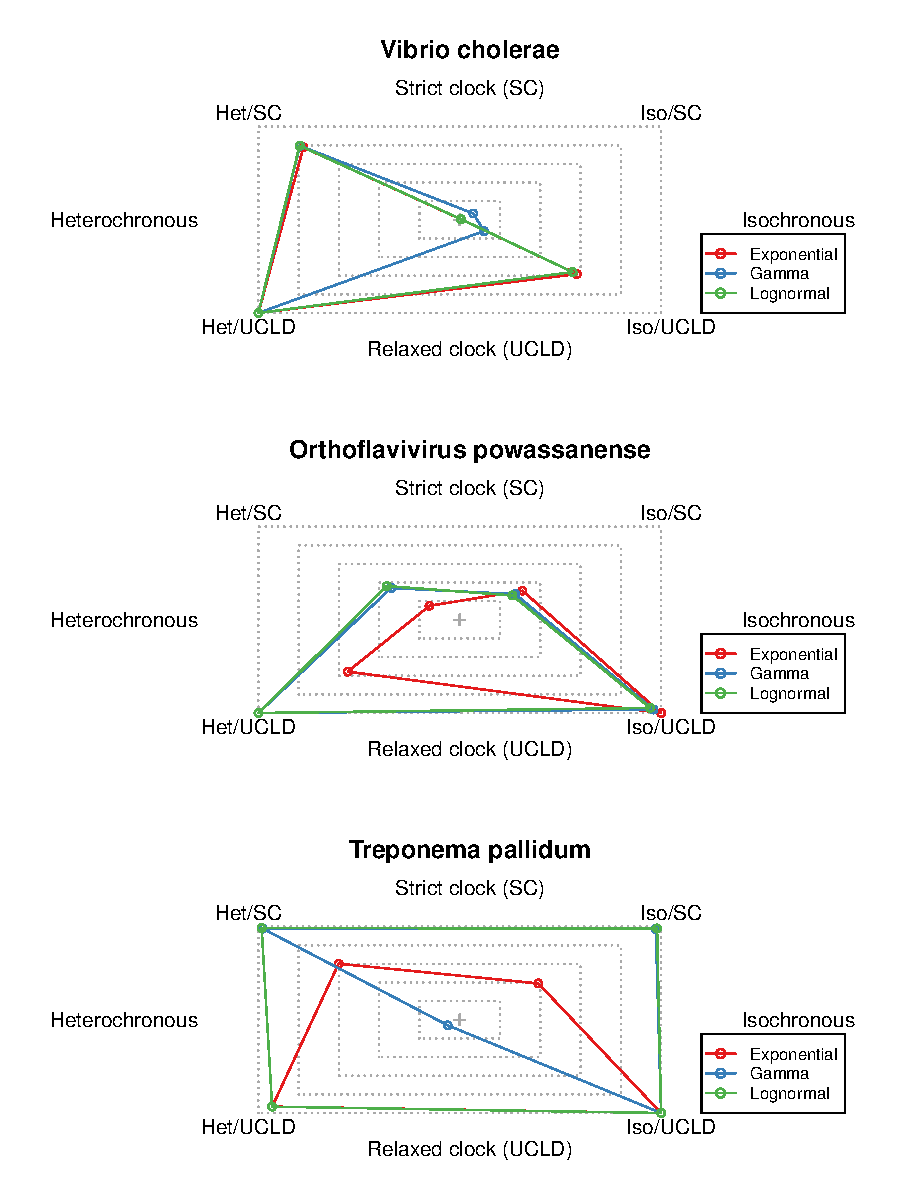
\includegraphics[width=14cm]{sandbox_figures/polygon_plot.pdf}\newline
		\vspace{-0.5cm}
		\caption{\textbf{Relative log marginal likelihoods of empirical data sets}. The polygons represent the relative log marginal likelihoods of each microbe dataset under a different effective population size ($\theta$) prior, analysed with four different configurations. Het (heterochronous) includes sampling, while iso (isochronous) does not include any sampling times. SC is strict clock and UCLD is the uncorrelated lognormal relaxed clock. Red represents an exponential hyperprior on the effective population size, blue is a $\Gamma$ hyperprior, and green is a log-normal hyperprior.}
		\label{figure:polygon_plots}
	\end{center}
\end{figure}

Our empirical data analyses overall demonstrate that the choice of prior has an impact on Bayesian model selection and support. In the case of the \textit{V. cholerae} data, the detection of temporal signal was relatively robust to the prior. Consistently, we found that the posterior distribution of key parameters such as the evolutionary rate was not very sensitive to the prior for this data set (Supplementary material). Moreover, this data set has been shown to have clear clocklike behaviour in root-to-tip regressions and date randomisation tests \cite{duchene2016genome}. In contrast, for the data sets of \textit{Powassan virus} and \textit{T. pallidum}, where temporal signal was not supported for all model configurations, we found that the posterior was more sensitive to the choice of prior (Supplementary information).

\subsection*{Simulation experiments}
To understand the impact of the prior on BETS results in more details, we conducted a set of simulation experiments where the data generating process is well understood. We conducted simulations under four possible conditions: a strict or relaxed molecular clock, and where the phylogenetic time-trees were heterochronous or isochronous. Data from heterochronous trees are sampled from a measurably evolving population and are expected to display temporal signal, whereas those from isochronous trees are not from a measurably evolving population (the time-trees are ultrametric) and should not display temporal signal. 

For data generated under heterochronous time-trees, we found that ten out of ten simulation replicates were correctly classified as having temporal signal, using a log Bayes factor of at least 3.2 (Table \ref{table:heterochronous_simulations_unbounded} and Fig \ref{figure:heterochronous_polygons}). This perfect classification, which can be considered a low type II error (where a type II error is failing to support temporal signal when it is truly present), was supported regardless of the prior on $\theta$ and the molecular clock model. 

\begin{table}[h!]
	\caption{\textbf{Correctly classified simulation replicates under heterochronous trees.} A total of ten simulations were generated in each case, under heterochronous trees, such that they are expected to display temporal signal. A number of ten represents perfect classification according to the Bayesian evaluation of temporal signal, BETS and a log Bayes factor of at least 3.2 (strong evidence for temporal signal). The rows correspond to three possible priors on the effective population size of the constant-size coalescent, $\theta$. The `Best clock model' is a situation where we consider the best heterochronous and isochronous model, take their log Bayes factor, and determine temporal signal if it is at least 3.2.}
	\begin{center}
		\label{table:heterochronous_simulations_unbounded}
		\begin{tabular}{| c + c | c | c |}
			\hline
			\multicolumn{1}{|c|}{\bf True clock model; clock model in analysis} & Exponential & $\Gamma$ & Log-normal\\ \thickhline
			Strict clock; Strict clock     & 10 & 10 & 10 \\ \hline
			Strict clock; Relaxed clock    & 10 & 10 & 10 \\ \hline
			Strict clock; Best clock model & 10 & 10 & 10 \\ \hline
			Relaxed clock; Strict clock    & 10 & 10 & 10 \\ \hline
			Relaxed clock; Relaxed clock    & 10 & 10 & 10 \\ \hline
			Relaxed clock; Best clock model & 10 & 10 & 10 \\ \hline		
		\end{tabular}
	\end{center}
\end{table}

\begin{figure}[!h]
	\begin{center}
		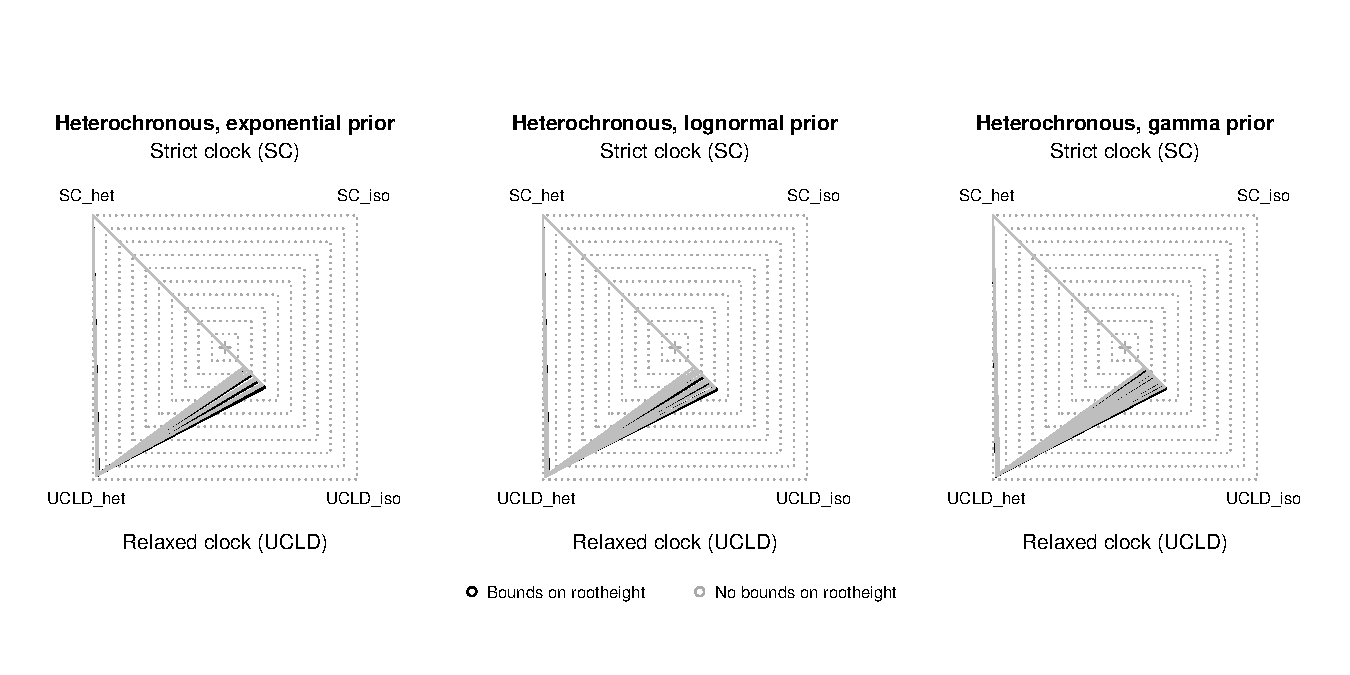
\includegraphics[width=14cm]{sandbox_figures/het_sims.pdf}\newline
		\vspace{-0.5cm}
		\caption{\textbf{Relative log marginal likelihoods of simulations with temporal signal.} The polygons represent the relative log marginal likelihood under three possible priors on the effective population size ($\theta$) parameter of the constant-size coalescent tree prior. Each corner corresponds to a combination of model and sampling times, either a strict (SC) or relaxed molecular clock with an underlying log-normal distribution (UCLD), and with (heterochronous) or without (isochronous) sampling times. The correct model used to generate the data is the SC heterochronous. Each polygon is for one simulation replicate (a total of ten) and the colours denote whether we employed a hard bound on the root height of the form Uniform(0.0, 5.0), in blue, or not, in orange.} 
		\label{figure:heterochronous_polygons}
	\end{center}
\end{figure}

For our data generated under isochronous trees, which by definition have no temporal signal, we found perfect classification under the exponential prior on $\theta$ under both clock models (Table \ref{table:isochronous_simulations_unbounded} and Fig \ref{figure:ultrametric_polygons}). For most analyses under the $\Gamma$ and log-normal priors on $\theta$ we found that BETS incorrectly supported the presence of temporal signal. The exceptions were for analyses of data analysed under a relaxed clock, whether they were simulated under a strict or relaxed clock. 

A perplexing result occurs under the best molecular clock model for the $\Gamma$ and log-normal priors on $\theta$. Here we take the log Bayes factor of the best heterochronous model vs the best isochronous model, which produced an increase in the classification error, relative to using the relaxed clock only. This phenomenon occurs because the incorrect inclusion of sampling times can mislead molecular clock model selection. As a case in point one of the simulation replicates under a relaxed molecular clock and an isochronous tree (with no temporal signal) had the following log marginal likelihoods; -4109.87 for the heterochronous analyses with a strict clock, -4117.06 for the isochronous analyses with a strict clock, -4124.35 for the heterochronous analyses with a relaxed clock, and -4118.29 for the isochronous analyses with a relaxed clock. The log Bayes factors under the relaxed clock have strong evidence against temporal signal (log Bayes factor=-6.06 for heterochronous vs isochronous), whereas the opposite is true for the strict clock (log Bayes factor=7.19). However, the best heterochronous model has substantially stronger support than the best isochronous model (here the strict or relaxed molecular clock, whose log marginal likelihoods differ by only 1.3 units). It is also worthwhile to note that in general, analyses under the relaxed clock tended to have fewer classification errors (for data sets with no temporal signal) than the strict clock, regardless of the true molecular clock model used to generate the data.

\begin{table}[h!]
	\caption{\textbf{Correctly classified simulation replicates under isochronous trees.} A total of ten simulations were generated in each case, under isochronous trees, such that they are not expected to support temporal signal. A number of ten represents perfect classification according to the Bayesian evaluation of temporal signal, BETS and a log Bayes factor of at most -3.2 (strong evidence against temporal signal). The rows correspond to three possible priors on the effective population size of the constant-size coalescent, $\theta$. The `Best clock model' is a situation where we consider the best heterochronous and isochronous model, take their log Bayes factor, and determine a lack of temporal signal if it is at most -3.2.}
	\begin{center}
		\label{table:isochronous_simulations_unbounded}
		\begin{tabular}{| c + c | c | c |}
			\hline
			\multicolumn{1}{|c|}{\bf True clock model; clock model in analysis} & Exponential & $\Gamma$ & Log-normal\\ \thickhline
			Strict clock; Strict clock     & 10 & 0 & 0 \\ \hline
			Strict clock; Relaxed clock    & 10 & 10 & 10 \\ \hline
			Strict clock; Best clock model & 10 & 0 & 0 \\ \hline
			Relaxed clock; Strict clock    & 10 & 0 & 0 \\ \hline
			Relaxed clock; Relaxed clock    & 10 & 9 & 9 \\ \hline
			Relaxed clock; Best clock model& 10 & 0 & 1 \\ \hline		
		\end{tabular}
	\end{center}
\end{table}

\begin{figure}[!h]
	\begin{center}
		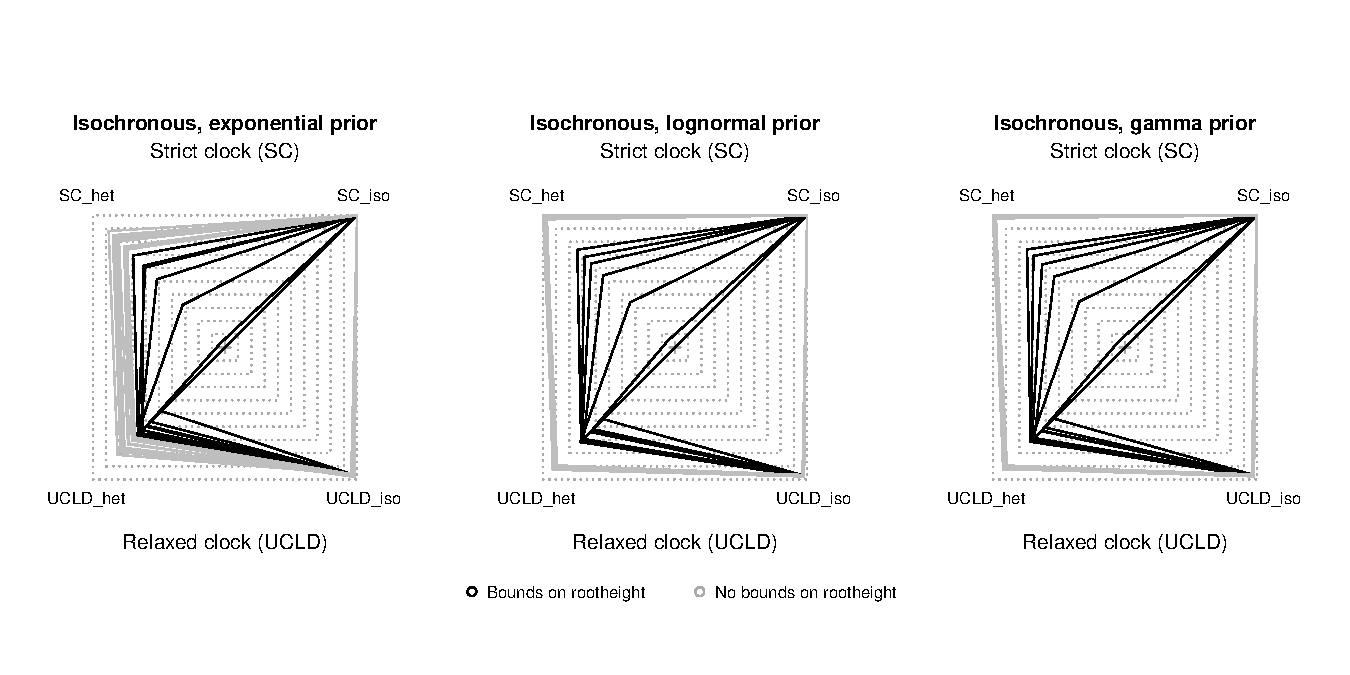
\includegraphics[width=14cm]{sandbox_figures/iso_sims.pdf}\newline
		\vspace{-0.5cm}
		\caption{\textbf{Relative log marginal likelihoods of simulations with no temporal signal.} The polygons here represent the same information as in Fig \ref{figure:heterochronous_polygons}. The correct model used to generate the data here is the SC isochronous (ultrametric).} 
		\label{figure:ultrametric_polygons}
	\end{center}
\end{figure}

Our simulation results demonstrate that detecting temporal signal when it is not present, which is akin to a type I error, is more common under some prior configurations (here the $\Gamma$ and log-normal priors on $\theta$) than the opposite (failing to detect temporal signal when it is present). Upon inspecting the resulting phylogenetic trees and the posterior of key parameters we found a probable cause. The incorrect inclusion of sampling times produces a dramatic overestimation of the height of the tree, especially under the strict molecular clock model, a phenomenon that we refer to as `tree extension' (Fig \ref{figure:ultrametric_tree_distortion}). Under this situation, the sampling times represent such a small proportion of the root height (the time from the most recently sampled node and the root-node), that the heterochronous tree is indistinguishable from one that is ultrametric and thus their log marginal likelihoods can be similar. In fact, the sampling times here spanned at most 0.5 units of time, such that they represent only 0.05\% of the total height of a tree height of 1,000, which is not unusual when there is tree extension. Moreover, the inclusion of sampling times may improve the fit of the model by accommodating natural stochasticity in the root-to-tip distances. The phenomenon of tree extension also occurs under the relaxed molecular clock, but to a much lesser extent, and thus under this model it is easier to correctly classify isochronous data sets. The exponential tree prior favour shallower trees and this is probably the reason for why results in more accurate classification.

\begin{figure}[h!]
	\begin{center}
		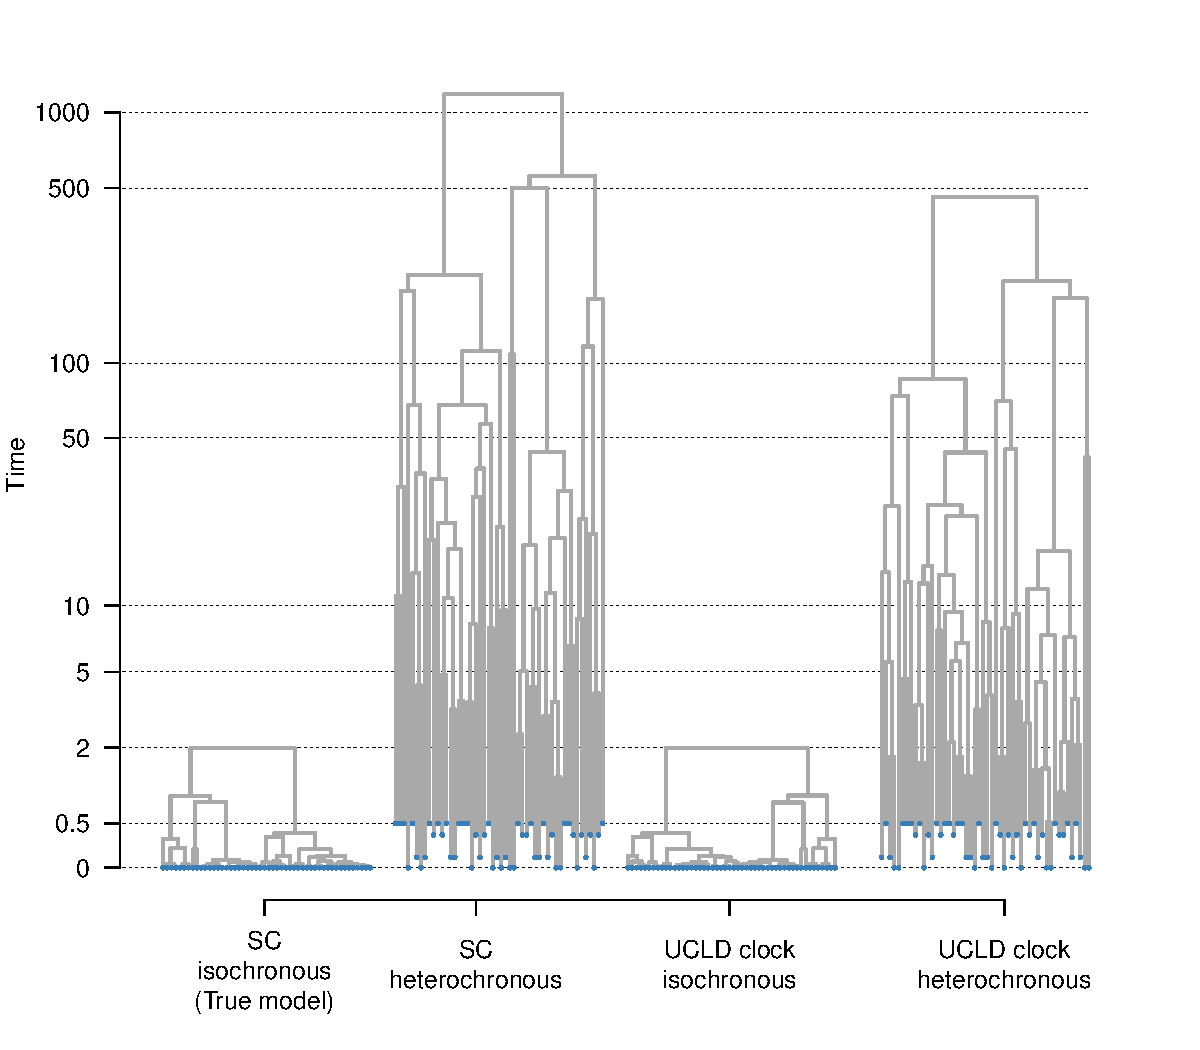
\includegraphics[width=15cm]{sandbox_figures/tree_distortion_ultrametric.pdf}\newline
		\vspace{-0.5cm}
		\caption{\textbf{Phylogenetic tree extension for a simulation replicate with no temporal signal}. Highest clade credibility trees from a data set simulated with no sampling times (isochronous) and under a strict molecular clock model (SC). The prior on $\theta$ is a $\Gamma(\kappa=0.001, \theta=1000)$, which resulted in high classification errors using BETS. The y-axis is the time from the present. Tip nodes have solid grey circles. Including sampling times that span 0.5 units of time and about 1/4 of the true root height induces dramatic overestimation of the root height, compared to the true model (SC, isochronous). This effect  occurs under both molecular clock models, the SC and the relaxed molecular clock with an underlying log-normal distribution (UCLD), but it is markedly less pronounced in the UCLD. Note that the y-axis is in logarithmic scale (log$_{10}$).}
		\label{figure:ultrametric_tree_distortion}
	\end{center}
\end{figure}

In Fig \ref{figure:heterochronous_tree_distortion} we show an example of phylogenetic trees from a simulation replicate with temporal signal (heterochronous). Failing to include sampling times, as in isochronous analyses, results in trees that are of similar height, so the confounding effect that we observe in isochronous data sets above does not occur. This is because the time-scale of the isochronous trees is determined by the value used to fix the molecular clock rate, which we set to the true value used for simulation in this case. When analysing empirical datasets for which this values is unknown, the typical approach is to fix this parameter to 1.0, which means that genetic distances are equal to the time of evolution. An important aspect of this method is that the $\theta$ parameter of the constant-size coalescent is proportional to units of time \cite{ho2011skyline, drummond2002estimating} (as are most other parameters of the tree prior, for example the growth rate of the exponential-growth coalescent). When time-calibrations are used $\theta$ is the population size multiplied by the generation time ($N_e \times$ generation time). Thus, the prior on $\theta$ for the heterochronous and isochronous analyses has different meanings, unless this parameter is scaled to match the units of the branch lengths, or the molecular clock rate in the isochronous analyses is fixed to a plausible value. In our simulations we fixed the molecular clock rate to its true value, but we also found that using a number within the expected order of magnitude of the organism in question is sufficient (e.g. 10$^{-4}$ to 10$^{-3}$ subs/site/year for a ssRNA virus).

\begin{figure}[!h]
	\begin{center}
		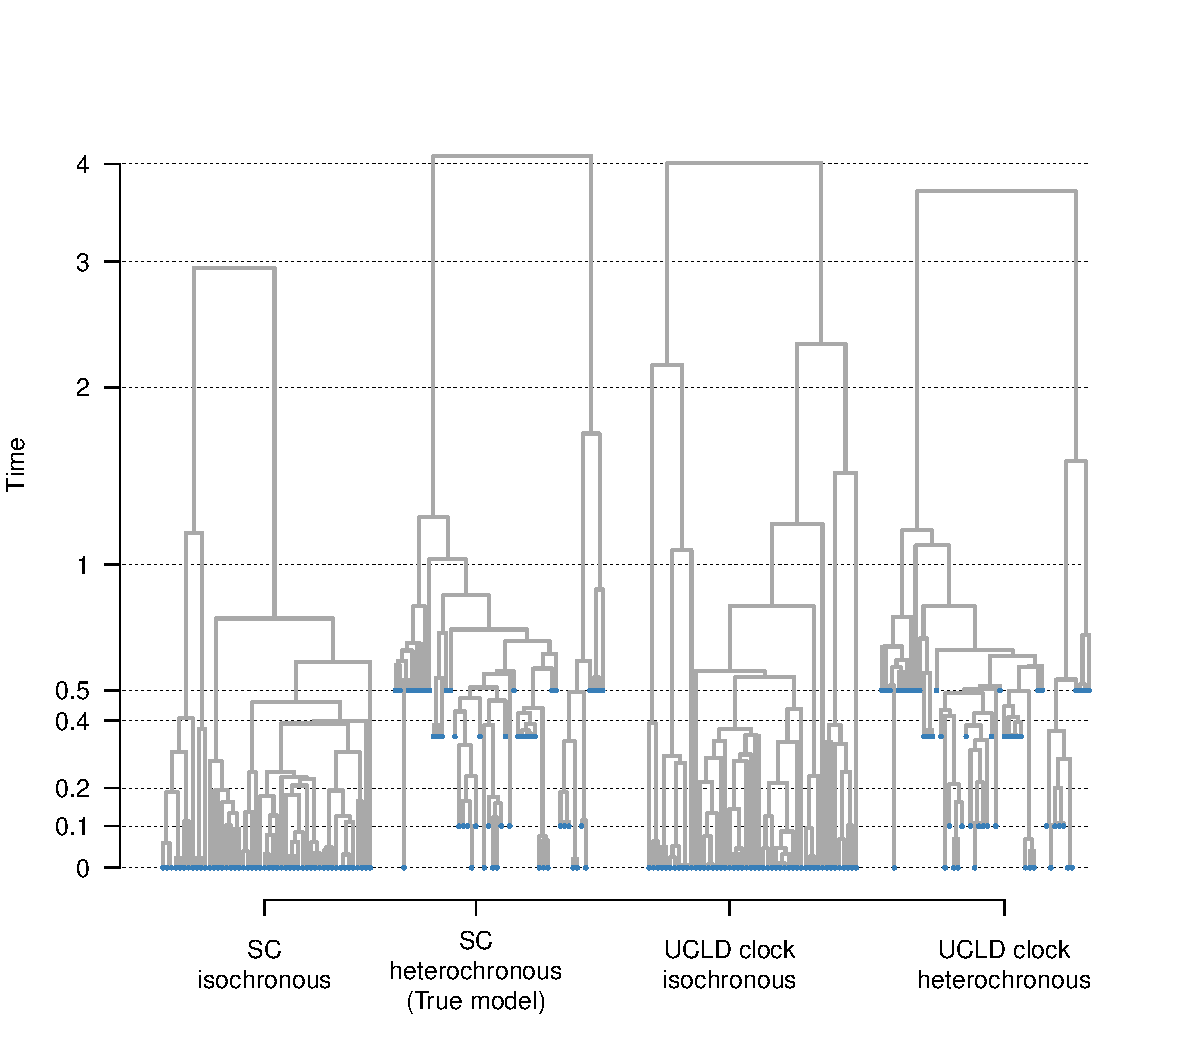
\includegraphics[width=15cm]{sandbox_figures/tree_distortion_heterochronous.pdf}\newline
		\vspace{-0.5cm}
		\caption{\textbf{Phylogenetic trees from a simulation replicate with temporal signal}. Highest clade credibility trees from a data set simulated with sampling times (heterochronous) and under a strict molecular clock model (SC). The isochronous trees are inferred by fixing the molecular clock rate to the true value, such that the time-scale is in the comparable units to the heterochronous analyses. Unlike the estimates for isochronous trees (e.g. Fig \ref{figure:ultrametric_tree_distortion}), the height of the trees  under all scenarios are comparable. Axes and labels are the same as those of Fig \ref{figure:ultrametric_tree_distortion}}
		\label{figure:heterochronous_tree_distortion}
	\end{center}
\end{figure}

Our results indicate that using priors favouring plausible node heights is important to ensure the accuracy of temporal signal detection. However, the interplay between the parameters of the tree prior and the resulting tree topologies and node heights is not necessarily trivial, particularly when the tree prior involves multiple parameters (e.g. the Bayesian skyride). Thus, defining suitable hyperpriors for the parameters of the tree prior requires careful attention. A pragmatic solution is to include additional prior information in the form of hard bounds on the root-height or the molecular clock rate. To this end, we investigated the effect of including a uniform prior between 0.0 and 5.0 units of time for the root height, meaning that trees that are older than 5.0 units have a prior probability of 0.0. Importantly, the trees under which we generated our simulations had root heights of around 2.0 units of time, and thus the hard bound of 5.0 allows for trees that are over twice as old as the truth. 

Setting hard bounds on the root height resulted in perfect classification accuracy for both, the heterochronous and isochronous simulation (Table \ref{table:heterochronous_simulations_bounded} and Fig \ref{figure:heterochronous_polygons}, and Table \ref{table:isorochronous_simulations_bounded} and Fig \ref{figure:ultrametric_polygons}, respectively). The improvement in classification for data sets with no temporal signal is likely because the hard bounds limit the tree extension phenomenon and thereby including sampling times imposes a penalty on the log marginal likelihood (see polygons in Fig \ref{figure:heterochronous_polygons}). Our empirical data set of \textit{V. cholerae}, which had evidence of temporal signal under all prior conditions, also displayed strong evidence for temporal signal with a hard bound on of 500 years before present on the root height (all log Bayes factors were at least 200 in favour of temporal signal).

\begin{table}[h!]
	\caption{\textbf{Correctly classified simulation replicates under heterochronous trees using hard bounds on the root height.} Rows and columns are identical to those of Table \ref{table:heterochronous_simulations_unbounded}, but here the heterochronous analyses include an explicit prior on the root height, via a uniform distribution between 0 and 5.0.}
	\begin{center}
		\label{table:heterochronous_simulations_bounded}
		\begin{tabular}{| c + c | c | c |}
			\hline
			\multicolumn{1}{|c|}{\bf True clock model; clock model in analysis} & Exponential & $\Gamma$ & Log-normal\\ \thickhline
			Strict clock; Strict clock     & 10 & 10 & 10 \\ \hline
			Strict clock; Relaxed clock    & 10 & 10 & 10 \\ \hline
			Strict clock; Best clock model & 10 & 10 & 10 \\ \hline
			Relaxed clock; Strict clock    & 10 & 10 & 10 \\ \hline
			Relaxed clock; Relaxed clock    & 10 & 10 & 10 \\ \hline
			Relaxed clock; Best clock model & 10 & 10 & 10 \\ \hline		
		\end{tabular}
	\end{center}
\end{table}

\begin{table}[h!]
	\caption{\textbf{Correctly classified simulation replicates under isochronous trees using hard bounds on the root height.} Rows and columns are identical to those of Table \ref{table:isochronous_simulations_unbounded}, but here the heterochronous analyses include an explicit prior on the root height, via a uniform distribution between 0 and 5.0.}
	\begin{center}
		\label{table:isorochronous_simulations_bounded}
		\begin{tabular}{| c + c | c | c |}
			\hline
			\multicolumn{1}{|c|}{\bf True clock model; clock model in analysis} & Exponential & $\Gamma$ & Log-normal\\ \thickhline
			Strict clock; Strict clock     & 10 & 10 & 10 \\ \hline
			Strict clock; Relaxed clock    & 10 & 10 & 10 \\ \hline
			Strict clock; Best clock model & 10 & 10 & 10 \\ \hline
			Relaxed clock; Strict clock    & 10 & 10 & 10 \\ \hline
			Relaxed clock; Relaxed clock    & 10 & 10 & 10 \\ \hline
			Relaxed clock; Best clock model& 10 & 10 & 10 \\ \hline		
		\end{tabular}
	\end{center}
\end{table}

\subsection*{Prior predictive simulations and parameter correlations}
We simulated phylogenetic trees from a prior distribution to inspect the correlation of parameters and the marginal prior for those that have obvious associations (e.g. the evolutionary rate has a CTMC-rate reference prior that depends on tree length). These simulations are commonly known as prior predictive simulations (e.g. \cite{wesner2021choosing}), and referred to in the phylogenetic literature as `sampling from the prior' \cite{nascimento2017biologist}. Initially, we set a uniform prior on $\theta$ from 0 to 10$^3$ and recorded the evolutionary rate, the tree length and root height. This prior is not generally recommended \cite{bouckaertDating}, and we present it here to illustrate correlations between parameters and the marginal prior, instead of using it for analysing our data.

An obvious finding is a natural positive correlation between tree length, root height, although the trends is not strictly linear (Fig \ref{figure:correlation_plots}). We also observed a positive correlation between $\theta$, tree length and tree height, which is expected because large population sizes impose long coalescent times \cite{rosenberg2002genealogical}. The nature of this correlation is heteroskedastic, with the variance in these tree statistics increasing with $\theta$. Our simulations demonstrate an inverse relationship between the evolutionary rate, $\theta$ and the tree statistics, but with a range that can span several orders of magnitude and with values ranging from 10$^{-9}$ to 10$^{-4}$ subs/site/time, meaning that the CTMC-rate reference prior tends to be diffuse. It is also noteworthy that the uniform prior on $\theta$ does not result in uniform marginal prior distributions for any of the parameters investigated here.

\begin{figure}[!h]
		\begin{center}
		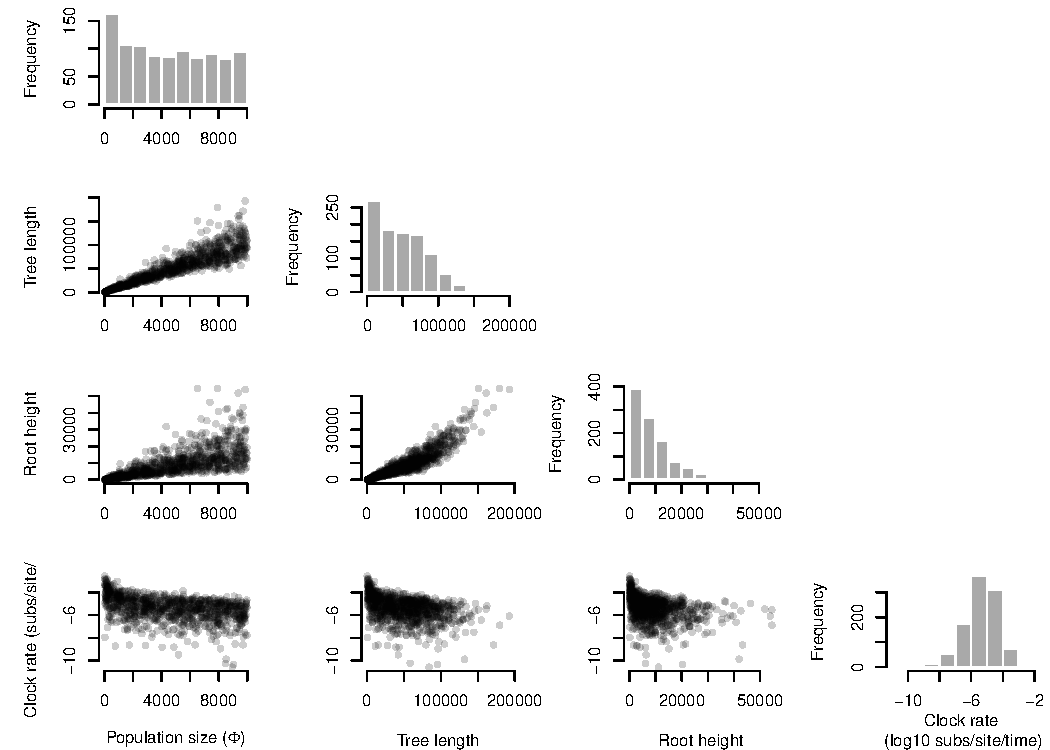
\includegraphics[width=14.7cm]{sandbox_figures/prior_predictive_plots.pdf}\newline
		\vspace{-0.5cm}
  \newline
		\caption{\textbf{Marginal prior distributions and pairs plots.} The grey histograms for correspond to the parameter labelled at the bottom of each column; effective population size (pop. size, $\theta$), tree length, root height, and the evolutionary rate (evol. rate). The prior for $\theta$ here is a Uniform distribution between 0 and 10$^3$, while that for the evolutionary rate is a CTMC-rate reference prior. Note that the tree length and root height have units of time, the evolutionary rate is in subs/site/time, and $\theta$ is proportional to units of time. }
        \label{figure:correlation_plots}
		\end{center}
\end{figure}

We conducted prior predictive simulations for the six prior configurations for $\theta$ under a heterochronous data set. In Fig \ref{figure:prior_tree_distros} we show the resulting distribution on the root height. The exponential ($\theta \sim Exponential(\mu=1.0)$, $\Gamma$ ($\Gamma(\kappa=0.001, \theta=1000)$) and log-normal (log-normal$(\mu=1.0, \sigma=5.0)$) prior distributions respectively produced mean root heights of 2.90 (95\% quantile range, qr: 1.62 to 14.34), 1.61 (95\% qr: 1.50 to 4.87) and 772.11 (95\% qr: 1.66 to $5.06 \times 10^5$) units of time. Clearly, the log-normal is the most vague prior here, but it produces implausible values of several orders of magnitude higher than our expectation of tree heights of around one and ten units of time (as simulated using $\theta=1.0$).

For comparison, we also simulated trees under the same priors on $\theta$ and with hard bounds on the root height with a uniform distribution with minimum and maximum values of 0.0 and 5.0, as described above. In this case, the exponential prior on $\theta$ yielded trees with root heights of mean 2.47 (95\% qr: 1.62 to 5.16), whereas those for the log-normal and $\Gamma$ were 1.61 (95\% qr: 1.50 to 5.11), and 1.96 (95\% qr: 1.54 to 4.42), respectively. As a result, in the log-normal prior on $\theta$ the use of hard bounds on the root height resulted in much smaller root heights, with a smaller impact on the exponential and $\Gamma$ priors.

\begin{figure}[!h]
	\begin{center}
		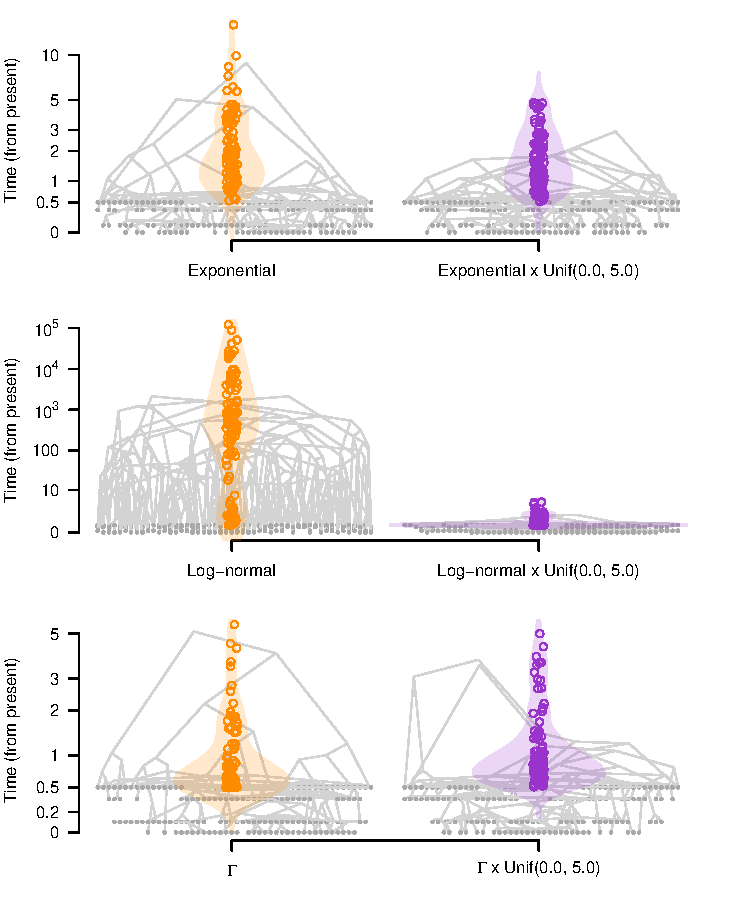
\includegraphics[width=13cm]{sandbox_figures/prior_tree_distros.pdf}\newline
		\vspace{-0.5cm}
		\caption{\textbf{Prior predictive simulations and marginal priors of root heights, given the prior on the effective population size, $\theta$}. Each panel corresponds to a different prior on $\theta$, as described on Table \ref{table:prior_distros_on_Phi} (Exponential($\mu=1.0$), Log-normal($\mu=$1.0, $\sigma=$5.0), and $\Gamma(\kappa=0.001, \theta=1000)$). We show five simulated trees from our analysis using sampling times (heterochronous analyses) and overlaid them (similar to densitree plots \cite{bouckaert2010densitree}). The violin plots show the prior densities of the root height and the hollow circles denote 100 randomly drawn samples from the prior. The y-axis is the time from the present, but note that the scales are different. Tip nodes are shown with solid grey circles. The densities and trees on the left, in orange, do not include an explicit prior on the root height ($T_h$), while those to the right, in purple, have a hard bound on tree height in the form of a uniform prior between 0.0 and 5.0 units of time.}
		\label{figure:prior_tree_distros}
	\end{center}
\end{figure}

\section*{Discussion}
Our study demonstrates that the choice of prior distribution has an impact on Bayesian model selection and that it can mislead tests of temporal signal. In general, data sets with no temporal signal are easily misclassified when the prior favours an implausibly old root height and low evolutionary rates, resulting in type I errors. In turn, incorrectly detecting temporal signal appears to result in a systematic overestimation of the evolutionary timescale and an underestimation of the molecular clock rates. 

We find that tree extension is the most probable reason for the incorrect detection of temporal signal in BETS, because it reduces the sampling window relative to the root height, such that the trees with sampling times are very similar to ultrametric trees. The phylogenetic likelihood of such overly old trees can be consistent with that from much shallower trees with no sampling times if their evolutionary rate is very low, such that the genetic distance along their branches is comparable. While the phenomenon of tree extension occurs for the strict and relaxed molecular clock models, it is less pronounced in the relaxed molecular clock model (e.g. see Fig \ref{figure:ultrametric_tree_distortion}). A probable reason for why the relaxed molecular clock is more robust to tree extension in data sets that are truly isochronous is that this model can absorb the incorrect inclusion of sampling times by treating them as rate variation among lineages.

The presence, rather than the absence, of temporal signal is much easier to detect, meaning low type II errors. In this case, specifying an incorrect isochronous model does not result in an obvious distortion of the time tree that could mislead BETS, at least under the conditions that we used here. It is conceivable, however, that certain priors on the phylogenetic tree or evolutionary rate could result in type II errors. 

Careful prior elicitation appears important for Bayesian model selection (see \cite{bergsten2013bayesian} for a similar problem in topology tests). Our results point to several recommendations to improve tests of temporal signal. First, the parameters of the tree prior for isochronous and heterochronous analyses should be in the same units of time, which facilitates comparison of the models in question. For example, fixing the evolutionary rate to 1.0 in an isochronous analysis means that branch lengths are in units of subs/site and thus the coalescent parameters have a different meaning to those estimated under heterochronous analyses (where the evolutionary rate is a free parameter). A more tractable approach is to conduct isochronous analyses by fixing the evolutionary rate to a value in the expected order of magnitude. Biological knowledge, such as the negative correlation between genome size and rates of microbes \cite{sanjuan2012molecular, duchene2016genome} or simply a previous estimate for a closely related organism, can be helpful for specifying such values. 

A second important recommendation is to conduct prior predictive simulations. As we show here, they are essential to understand potential interactions between model parameters and ultimately whether the prior expectation is reasonable with respect to our knowledge about the data. In our simulation study, using hard bounds on the tree height alleviated the problem of tree extension when the prior on $\theta$ favoured very old trees. In empirical data, however, one may not want to make such strong statements, and prior predictive simulations can help determine whether the tree prior and associated parameters produce trees with sensible root heights (e.g. the exponential prior on $\theta$ had low type I and type II errors in our simulations). Finally, prior sensitivity analyses can be useful to determine the extent to which the prior can influence the posterior \cite{foster2017evaluating, lopes2011confronting}, and model selection using Bayes factors \cite{lambert2018student}. A prior that makes unreasonable statements and is overly influential on the posterior should be considered carefully. The exponential prior on $\theta$ in the \textit{Powassan virus} did not support temporal signal, but note that it is much more influential on the posterior than the $\Gamma$ and log-normal priors for this particular data set. In contrast, the \textit{V. cholerae} data seemed robust to the three priors that we used. Some empirical data sets yielded unclear evidence for temporal signal according to BETS, such as the \textit{T. pallidium} data set that we reanalysed. In such cases, current practice is to consider multiple lines of evidence, including date-randomisation tests \cite{duchene2015performance, ramsden2009hantavirus}, comparisons of the prior and posterior \cite{duchene2020estimating}, and root-to-tip regressions.\cite{featherstone2023clockor2, rambaut2016exploring}. 

%Although this approach seems appropriate, the fully Bayesian nature of BETS means that it is straight-forward to incorporate additional information that may be key for obtaining temporal signal. In the study that described the \textit{T. pallidium} data set, the authors conducted their Bayesian analyses with monophyletic constraints that enforced a particular position for the root node, based on independent information \cite{majander2020ancient}, and obtained sensible results and strong temporal signal, according to a date-randomisation test. Our finding that this data set had unclear temporal signal in the absence of such constraints indicates that such additional information should be considered, where possible.

The sum of our results and recommendations has implications for the reliability of estimates of evolutionary rates and time-scales, for determining whether a population is measurably evolving, and for assessing the phylodynamic threshold of emerging microbes. This concept refers to the point in time when a microbe has accumulated a sufficient amount of evolutionary change to enable phylogenetic estimates of its emergence time \cite{duchene2020temporal}. Concretely, genome data from recently emerging microbes may have very few substitutions, in which case prior sensitivity analyses and prior predictive simulations would easily reveal whether the data are sufficiently informative. Overall, tests of temporal signal have a key place in genomic analyses of pathogens and our results will be useful as guidelines to improve their application and interpretation.

\section*{Materials and methods}
\subsection*{Empirical data}
We selected three different datasets to evaluate temporal signal, \textit{V. cholerae} \cite{devault2014second}, \textit{Powassan virus} \cite{vogels2023phylogeographic}, and \textit{T. pallidum} \cite{majander2020ancient}. These varied in their sampling timeframe, number of informative sites, and number of sequences. The most sparse dataset was \textit{T. pallidum}, where sampling dates spanned 481 years (1534 to 2016), with 28 sequences each containing 1,500 SNP sites. Among these samples, there were only two in the 1500's and two in the 1700's, with the rest of the samples concentrated in the 1900's to 2000's. There were 319 sequences with 11,193 sites (the complete genome) for \textit{Powassan virus}, spanning 24 years of sampling times (1995 to 2019). Most of the samples were collected after 2010, with only three isolated in 1995. For \textit{V. cholera} we had 122  sequences with 1,57 SNP sites across 73 years of sampling (1937 to 2010). There are 1,392 unique site patterns in \textit{V. cholera}, 3,457 in \textit{Powassan virus}, and 840 in \textit{T. pallidum}. %In the simulated data, there are 580-710 (SC) and 640-710 (UCLD) in cholera, and 110-150 in both SC and UCLD for treponema. For the \textit{Powassan virus} SC, there are $\sim$4800 in the isochronous trees and $\sim$14650 in the heterchronous trees.

For \textit{V. cholerae} and \textit{T. pallidum} our data consisted of SNP sites. To account for such ascertainment bias, we specified the number of constant sites of each nucleotide in our subsequent analyses. We sampled the posterior distribution using Markov chain Monte Carlo as implemented in BEAST1.10. The chain length was $10^8$ steps, sampling every $10^3$ to draw a total of $10^4$ samples. The prior for the evolutionary rate of the strict clock was a CTMC-rate reference prior (i.e. a $\Gamma(\alpha=0.5, \beta=$tree length, and mean=$\alpha/\beta$) \cite{ferreira2008bayesian}. For the log-normal distribution of the relaxed clock we also used the CTMC-rate reference prior for the mean rate (known as the ucld.mean in the program) and an exponential prior with mean 0.33 for the standard deviation (the ucld.stdev in the program). For the tree prior we used a constant-size coalescent with population size, $\theta$ with three possible priors, as described in Table \ref{table:prior_distros_on_Phi}. In all cases we used the HKY+$\Gamma_4$ substitution model, with the default priors in BEAST1.10.

To calculate log marginal likelihoods we used generalised stepping-stone \cite{baele2016genealogical,fan2011choosing}. This method requires a working distribution for all parameters, including the tree prior, for which we used the matching coalescent model. We set 100 path steps between the unnormalised posterior and the working distribution, following equally spaced intervals from a $\beta(0.3, 1.0)$ distribution. For each step we ran a chain length of 2$\times 10^{6}$ steps.

\subsection*{Simulation experiments}
For our simulations we considered well-understood conditions to isolate the impact of the tree prior on tests of temporal signal. We simulated phylogenetic trees under a constant-size coalescent model with a fixed population size of 1.0. The trees could be isochronous (i.e. ultrametric) or heterochronous. In the latter case we randomly assigned tip heights of of 0.0, 0.10, 0.35, or 0.50, with equal probability. This situation implies four discrete sampling periods, which resembles sequencing blitzes \cite{porter2022new}, or archaeological sampling of strata \cite{zhang2016total}. Because the coalescent model used to analyse the data conditions on sampling times we expect it to be robust to such sampling bias \cite{stadler2015well, volz2014sampling, featherstone2021infectious}. We used a JC substitution model \cite{jukes1969evolution} to generate sequence alignments of 1,000 nucleotides and an evolutionary rate of 0.05 subs/site/time, which resulted in around 250 unique site patterns. For our simulations under a relaxed molecular clock we sampled branch rates from a log-normal distribution with mean 0.05 and standard deviation of 0.25. The procedure for obtaining the simulated alignments consisted of specifying the model above in BEAST1.10 with an empty sequence alignment to sample phylogenetic trees. We then used NELSI \cite{ho2015simulating} and Phangorn \cite{schliep2011phangorn} to simulate evolutionary rates and sequence alignments, respectively.

We analysed the simulated data under heterochronous and isochronous models. For the heterochronous analysis we used the correct sampling times (where the correct model was the heterochronous) or assigned the tip heights above randomly (0.0, 0.10, 0.35, or 0.50) where the isocrhonous was the true model. For the evolutionary rate (clock.rate the strict and ucld.mean for the relaxed molecular clock model) we set the default CTMC-rate reference prior and the six possible configurations of the prior on $\theta$ (Table \ref{table:prior_distros_on_Phi}, plus those with hard bounds on the root height). For the isochronous analyses we did not specify sampling times and we fixed evolutionary rate to its true value of 0.05 to ensure that the branch lengths, $\theta$ and other parameters are in the correct units. We calculated log marginal likelihoods with the same procedure as for the empirical data.

\section*{Supporting information}
% Include only the SI item label in the paragraph heading. Use the \nameref{label} command to cite SI items in the text.

\paragraph*{S1 Fig.}
\label{S1_Fig}
	\begin{center}
		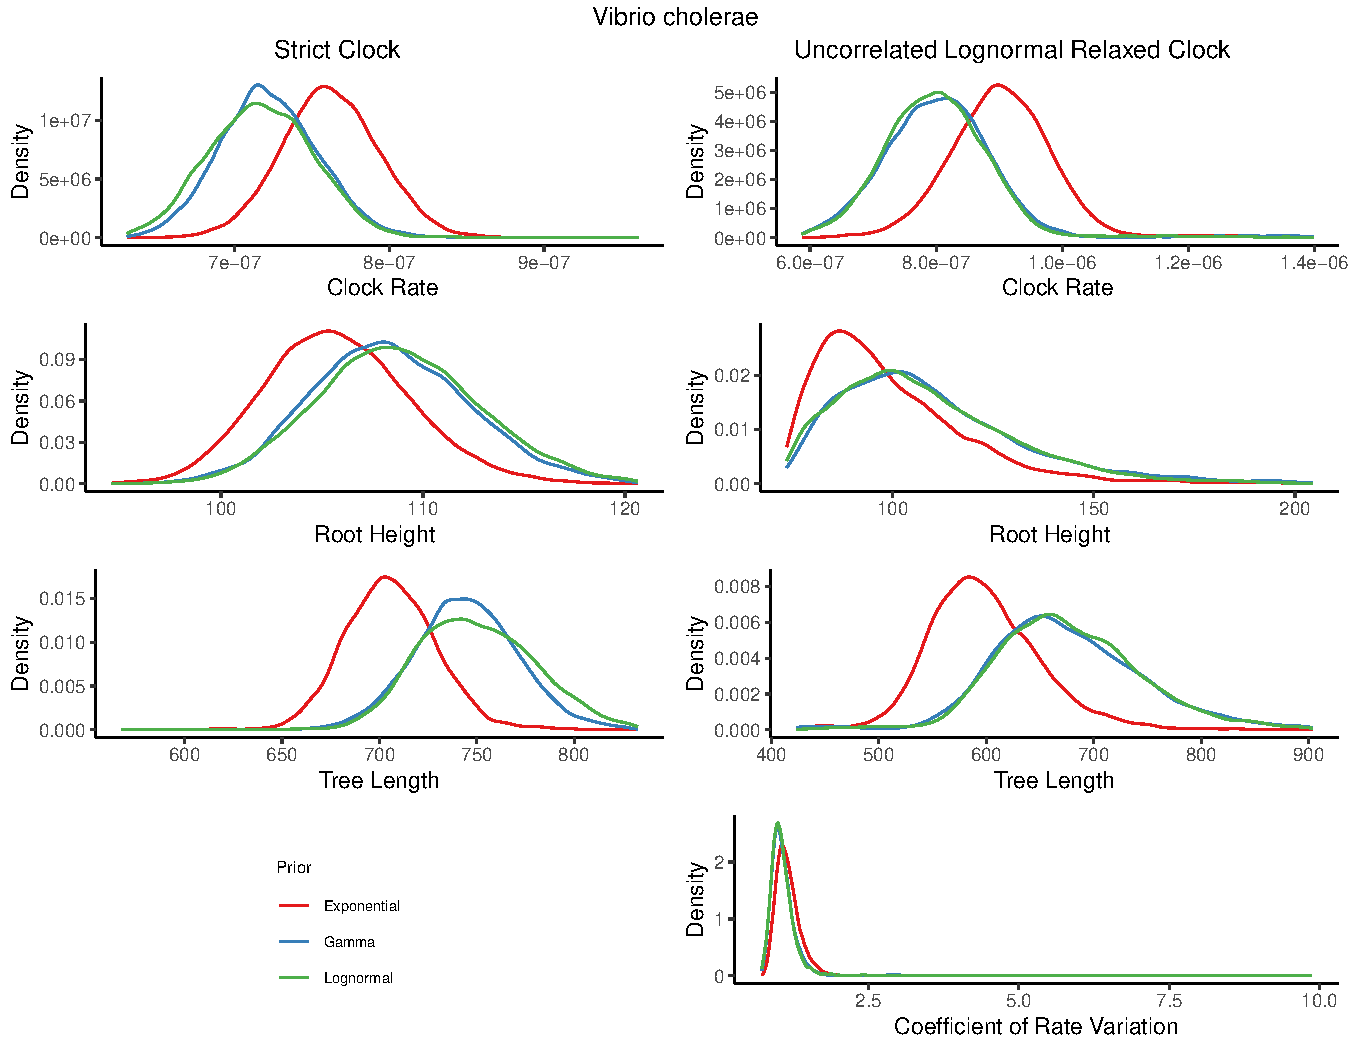
\includegraphics[width=13cm]{sandbox_figures/cholera_density_plot.pdf}\newline
		\textbf{Densities of key statistics of cholera empirical data.} The clock rate, root height, tree length, and coefficient of rate variation are shown under three priors on $\theta$, exponential (red), gamma (blue), and lognormal (green).
	\end{center}
\paragraph*{S2 Fig.}
\label{S2_Fig}
	\begin{center}
		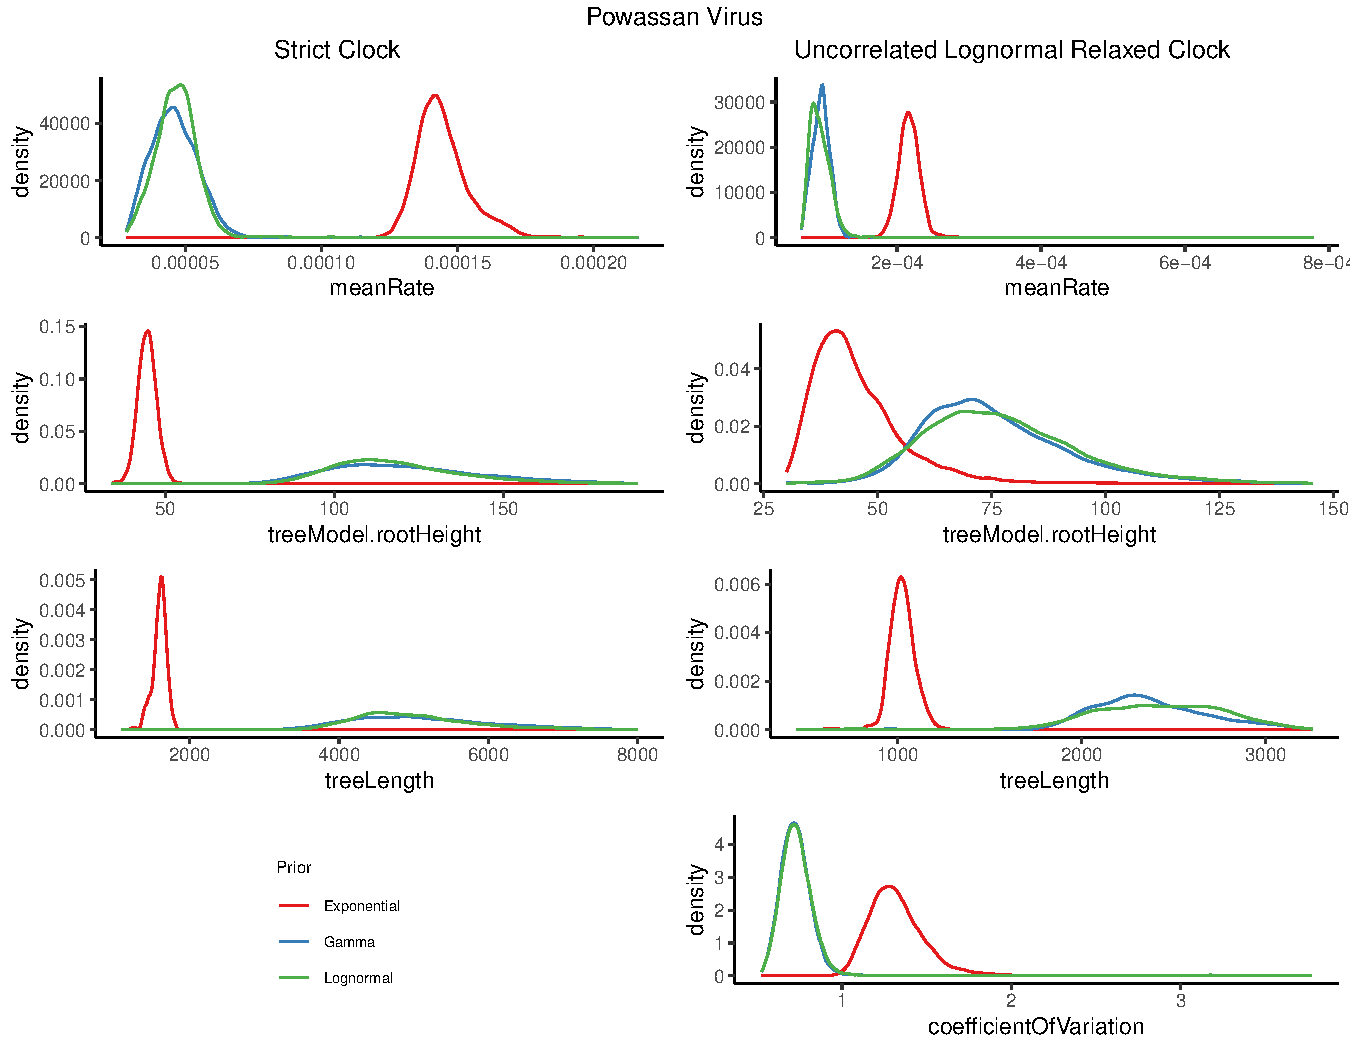
\includegraphics[width=13cm]{sandbox_figures/powv_density_plot.pdf}\newline
		\textbf{Densities of key statistics of \textit{Powassan virus} empirical data.} The clock rate, root height, tree length, and coefficient of rate variation are shown under three priors on $\theta$, exponential (red), gamma (blue), and lognormal (green).
	\end{center}
\paragraph*{S3 Fig.}
\label{S3_Fig}
	\begin{center}
		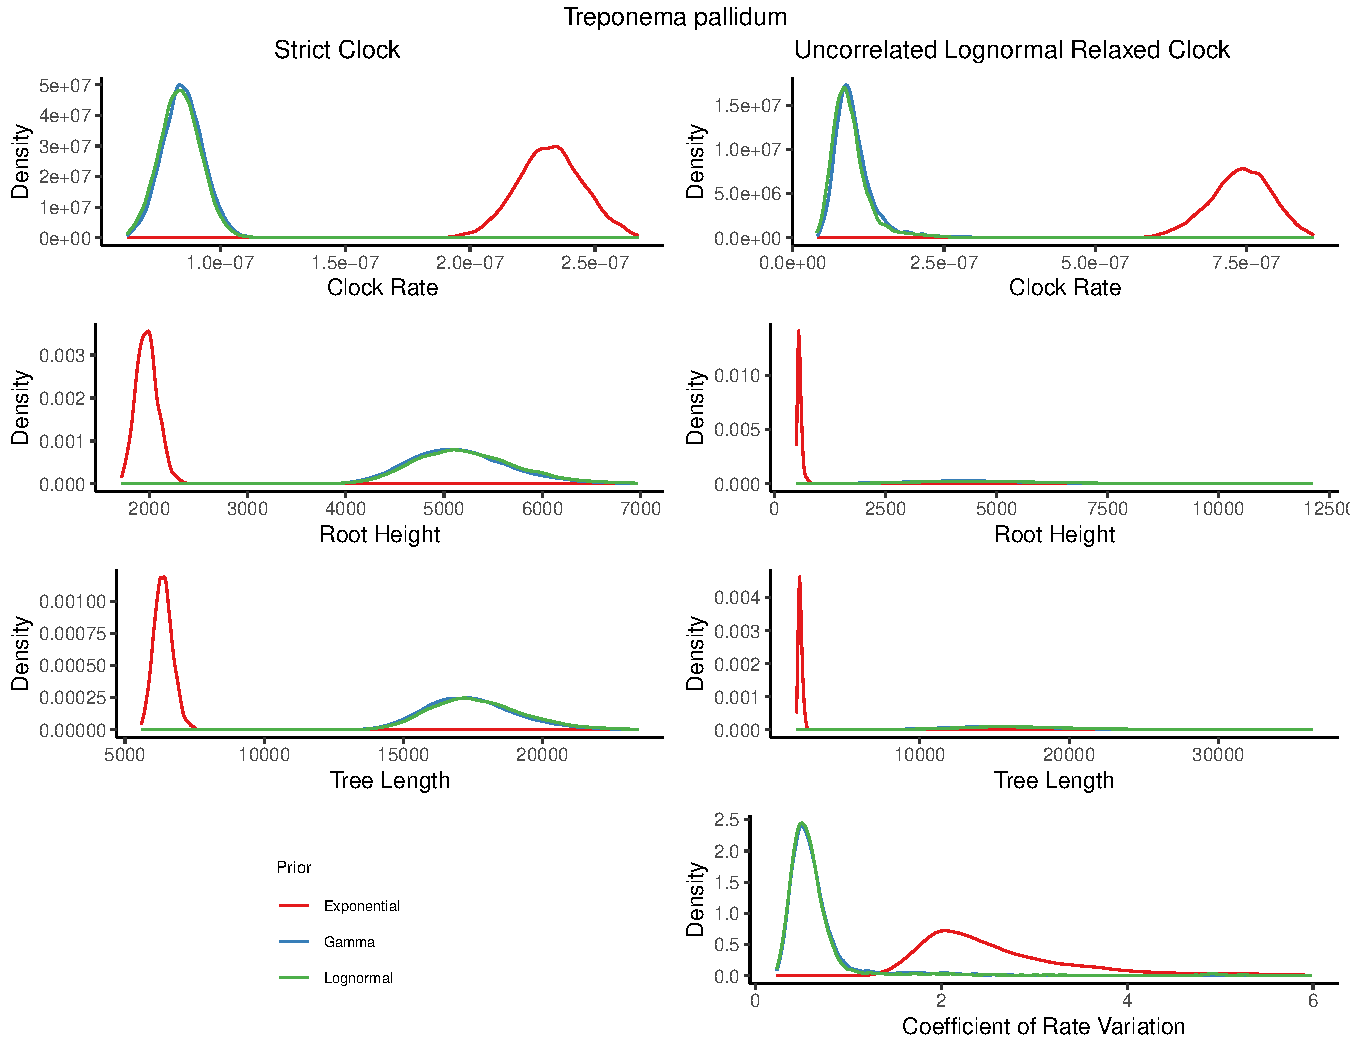
\includegraphics[width=13cm]{sandbox_figures/treponema_density_plot.pdf}\newline
		\textbf{Densities of key statistics of \textit{Treponema palladium} empirical data.} The clock rate, root height, tree length, and coefficient of rate variation are shown under three priors on $\theta$, exponential (red), gamma (blue), and lognormal (green).
	\end{center}
 \paragraph*{S4 Fig.}
\label{S4_Fig}
	\begin{center}
		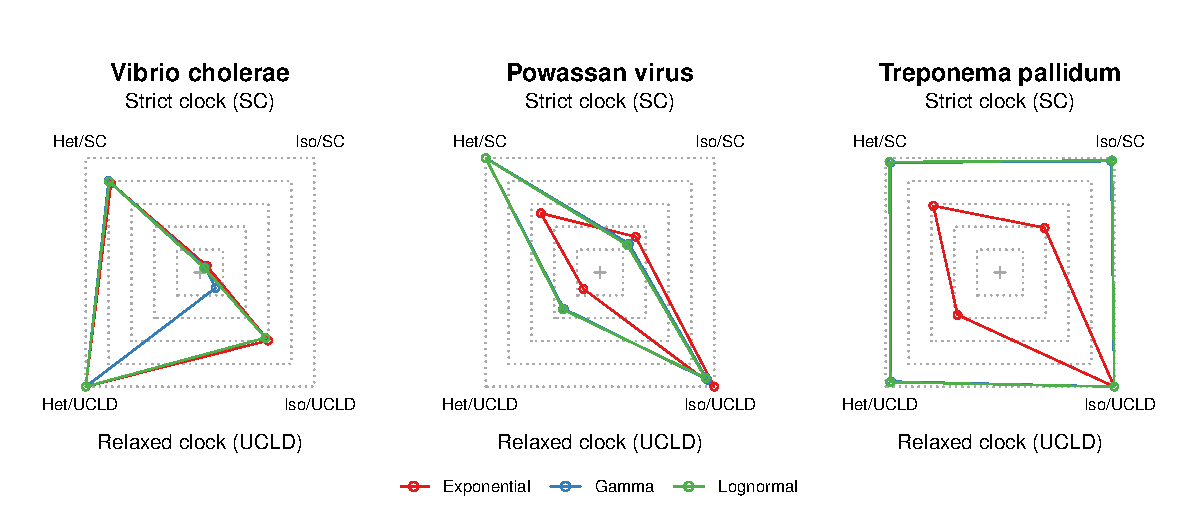
\includegraphics[width=13cm]{sandbox_figures/polygon_plot_bound.pdf}\newline
		\textbf{Relative log marginal likelihoods of empirical data sets with bounds on root height.} The polygons represent the relative log marginal likelihoods of each microbe dataset under a different effective population size ($\theta$) prior, analysed with four different configurations. Het (heterochronous) includes sampling, while iso (isochronous) does not include any sampling times. SC is strict clock and UCLD is the uncorrelated lognormal relaxed clock. Red represents an exponential hyperprior on the effective population size, blue is a $\Gamma$ hyperprior, and green is a log-normal hyperprior..
	\end{center}

\section*{Acknowledgments}
This work was supported by the Inception program [Investissement d’Avenir grant ANR-16-CONV-0005], the Australian National Health and Medical Research Council [2017284], and the Australian Research Council [FT220100629].

\nolinenumbers


% Either type in your references using
% \begin{thebibliography}{}
% \bibitem{}
% Text
% \end{thebibliography}
%
% or
%
% Compile your BiBTeX database using our plos2015.bst
% style file and paste the contents of your .bbl file
% here. See http://journals.plos.org/plosone/s/latex for 
% step-by-step instructions.
% 
%\begin{thebibliography}{10}
\bibliography{References}

%\bibitem{bib1}
%Conant GC, Wolfe KH.
%\newblock {{T}urning a hobby into a job: how duplicated genes find new
%  functions}.
%\newblock Nat Rev Genet. 2008 Dec;9(12):938--950.

%\bibitem{bib2}
%Ohno S.
%\newblock Evolution by gene duplication.
%\newblock London: George Alien \& Unwin Ltd. Berlin, Heidelberg and New York:
%  Springer-Verlag.; 1970.

%\bibitem{bib3}
%Magwire MM, Bayer F, Webster CL, Cao C, Jiggins FM.
%\newblock {{S}uccessive increases in the resistance of {D}rosophila to viral
%  infection through a transposon insertion followed by a {D}uplication}.
%\newblock PLoS Genet. 2011 Oct;7(10):e1002337.

%\end{thebibliography}



\end{document}

